\documentclass[12pt]{article}
\usepackage{mystyle}
\usepackage[T1]{fontenc}
\usepackage{mathptmx} % times new roman-ish 

\title{ECON899. 
Problem set 2}
\author{Emily Case, Hanna Han, Anna Lukianova}
\date{September 21, 2022}

\begin{document}
    \maketitle
    
\section*{Question I}
% NOTE: i am following Michael's stuff from last year and expanding:
% https://github.com/michaelnattinger/HOMEWORK/blob/master/Y2/Computational/PS2/PS2_nattinger_bass.pdf
% - emily 
Suppose we have the same model environment as in Huggett (1993) except that there are enforceable insurance markets regarding the idiosyncratic shocks to earnings and that there are no initial asset holdings. Note that this indicates we have complete markets.

Each household $i$ solves
\begin{align*}
    V = \max_{\{c_t^i\}_{t=0}^\infty} \sum_{t = 0}^\infty \beta^t u(c_t^i) \;\; \text{ s.t. } \;\; \sum_{t=0}^{\infty} q_t c_t^i \leq \sum_{t=0}^{\infty} q_t ( \mu + 0.5(1-\mu)) 
\end{align*}
Note that $\mu$ is the probability of a good shock (the agent is employed), and $1-\mu$ is the probability of a bad shock (the agent is unemployed).
% fraction of households that are employed.
% Anna: I have reformulated and added the summation sign.

The Lagrangian is 
\begin{align*}
    \mathcal{L} & =\sum_{t = 0}^\infty \beta^t u(c_t^i) - \lambda \left[ \sum_{t=0}^{\infty} q_t (c_t^i - \mu - 0.5(1-\mu)) \right]
\end{align*}
Then, the first order condition with respect to $c_t^i$ is 
\begin{align*}
    \beta^t u'(c_t^i) & = \lambda q_t 
\end{align*}
All households face the same preferences, which means $u'(c_t^i) = u'(c_t^j)$ and $c_t^i = c_t^j = c_t$. In order for the budget constraint to hold, it must be that
\[ c_t = \bar{c} = \mu + 0.5(1-\mu)\]
Next, we solve for $\lambda$ in order to relate the marginal utility of consumption today to that of tomorrow, noting that $u'(c_{t}) = u'(c_{t+1})$:
\begin{align*}
    \frac{\beta^t u'(c_t)}{q_t} & = \frac{\beta^{t+1}u'(c_{t+1})}{q_{t+1}} \\
    q_{t+1} \beta^t & = q_t \beta^{t+1} \\
    q_{t+1} & = q_t \beta 
\end{align*}
We normalize $q_0 = 1$, which means $q_t = \beta$. Therefore, the allocation in each period is $c_t = \bar{c}$ for all agents and the price in each period is $q_t = \beta$.
\\
\\
Plugging this back in means that value in period $t$ is $ V_t  = \sum_{t} \beta^t u(\mu + 0.5(1-\mu)) $ and $\mu$ will be equal to the probability a household is employed.
\\
\\
Then the first best welfare over all time of any household is 
\[ W^{FB} = \sum_t \beta^t u(c) = u(c) \sum_t \beta^t = \frac{u(c)}{1-\beta}\]
%
\section*{Question II}
\begin{enumerate}[label=(\alph*)]
    % Part (a)
    \item Figure \ref{fig:ii.a} shows the policy function $g(a,s)$.
    \begin{figure}[h!]
        \centering
        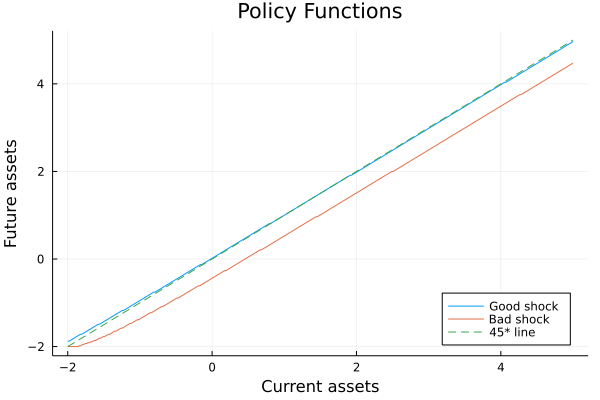
\includegraphics[width = 0.6\linewidth]{pset2/figures/PS2_Policy_Functions.png}
        \caption{Policy function $g(a,s)$}
        \label{fig:ii.a}
    \end{figure}
    
    % Part (b)
    \item The equilibrium bond price is 0.994287. Figure \ref{fig:ii.b} shows the  cross-sectional distribution of wealth for those employed and those unemployed. 
    \begin{figure}[h!]
        \centering
        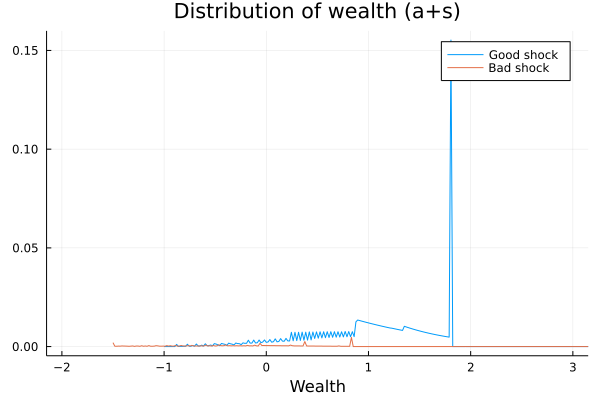
\includegraphics[width = 0.6\linewidth]{pset2/figures/PS2_Distribution.png}
        \caption{Cross-sectional distribution of wealth}
        \label{fig:ii.b}
    \end{figure}
    
    % Part (c)
    \item Figure \ref{fig:ii.c} shows the Lorenz curve. The Gini coefficient with respect to total wealth for the model economy is 0.408. From the Survey of Consumer Finances (SCF), we know that the Gini coefficient in the data is 0.80.
    \begin{figure}[h!]
        \centering
        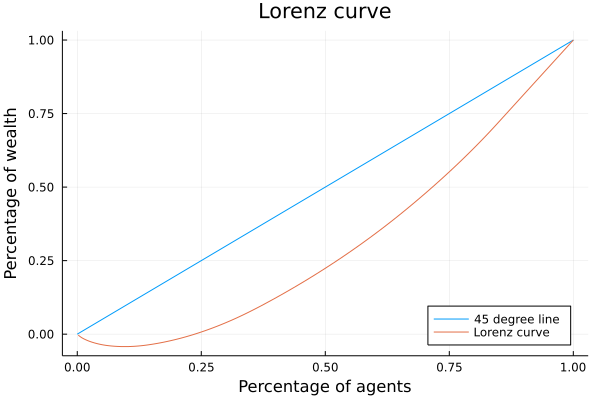
\includegraphics[width = 0.6\linewidth]{pset2/figures/PS2_Lorenz curve.png}
        \caption{Lorenz curve}
        \label{fig:ii.c}
    \end{figure}
\end{enumerate}
%
\section*{Question III}
\begin{enumerate}[label=(\alph*)]
    % Part (a)
    \item Figure \ref{fig:iii.a} plots the consumption equivalent $\lambda(a,s)$ across $a$ for both states $s \in \{e,u\}$.
    \begin{figure}[h!]
        \centering
        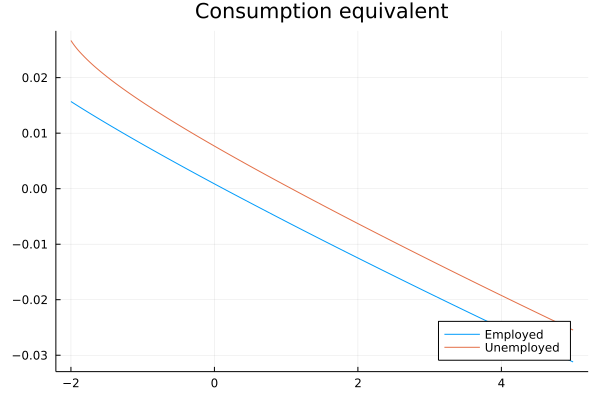
\includegraphics[width = 0.6\linewidth]{pset2/figures/PS2_IIIa.png}
        \caption{Consumption equivalent $\lambda(a,s)$}
        \label{fig:iii.a}
    \end{figure}
    
    % Part (b)
    \item We calculate $W^{FB}$, or the first-best aggregate welfare measure, using the results of the competitive equilibrium from Question I. We know that
        \begin{align*}
        W^{FB} &= \frac{U(c_t^i)}{1-\beta} \\[4pt]
        &= \frac{U(\bar{c})}{1-\beta} \\[4pt]
        &= \frac{U(\mu + 0.5(1-\mu))}{1-\beta} \\[4pt]
        &\approx-4.2525
        \end{align*}
    Next, we calculate $W^{INC}$, or the aggregate welfare measure for incomplete markets. We know that
        \begin{align*}
        W^{INC} &= \sum_{(a,s) \in A \times S} \mu(a,s) v(a,s) \\
        &\approx -4.4533
        \end{align*}
    Finally, we calculate $WG$, or the welfare gain, from switching to complete markets from incomplete markets. Then
        \begin{align*}
        WG &= \sum_{(a,s) \in A \times S} \lambda(a,s) \mu(a,s) \\
        &\approx 0.0014
        \end{align*}
    
    % Part (c)
    \item Agents whose consumption equivalent $\lambda(a,s) > 0$ would vote in favor of complete markets. As a result, 54.7\% of the population would vote in favor of complete markets.
\end{enumerate}
\end{document}